% Options for packages loaded elsewhere
\PassOptionsToPackage{unicode}{hyperref}
\PassOptionsToPackage{hyphens}{url}
%
\documentclass[
]{article}
\usepackage{amsmath,amssymb}
\usepackage{lmodern}
\usepackage{iftex}
\ifPDFTeX
  \usepackage[T1]{fontenc}
  \usepackage[utf8]{inputenc}
  \usepackage{textcomp} % provide euro and other symbols
\else % if luatex or xetex
  \usepackage{unicode-math}
  \defaultfontfeatures{Scale=MatchLowercase}
  \defaultfontfeatures[\rmfamily]{Ligatures=TeX,Scale=1}
\fi
% Use upquote if available, for straight quotes in verbatim environments
\IfFileExists{upquote.sty}{\usepackage{upquote}}{}
\IfFileExists{microtype.sty}{% use microtype if available
  \usepackage[]{microtype}
  \UseMicrotypeSet[protrusion]{basicmath} % disable protrusion for tt fonts
}{}
\makeatletter
\@ifundefined{KOMAClassName}{% if non-KOMA class
  \IfFileExists{parskip.sty}{%
    \usepackage{parskip}
  }{% else
    \setlength{\parindent}{0pt}
    \setlength{\parskip}{6pt plus 2pt minus 1pt}}
}{% if KOMA class
  \KOMAoptions{parskip=half}}
\makeatother
\usepackage{xcolor}
\usepackage{graphicx}
\makeatletter
\def\maxwidth{\ifdim\Gin@nat@width>\linewidth\linewidth\else\Gin@nat@width\fi}
\def\maxheight{\ifdim\Gin@nat@height>\textheight\textheight\else\Gin@nat@height\fi}
\makeatother
% Scale images if necessary, so that they will not overflow the page
% margins by default, and it is still possible to overwrite the defaults
% using explicit options in \includegraphics[width, height, ...]{}
\setkeys{Gin}{width=\maxwidth,height=\maxheight,keepaspectratio}
% Set default figure placement to htbp
\makeatletter
\def\fps@figure{htbp}
\makeatother
\setlength{\emergencystretch}{3em} % prevent overfull lines
\providecommand{\tightlist}{%
  \setlength{\itemsep}{0pt}\setlength{\parskip}{0pt}}
\setcounter{secnumdepth}{-\maxdimen} % remove section numbering
% \documentclass[14pt]{extarticle}

% page setup
% \usepackage[a4paper,
%             top=2.5cm,
% 			bottom=2.5cm,
% 			left=2.00cm,
% 			right=2.00cm,
% 			bmargin=2.50cm]{geometry}
\usepackage[a4paper,
			top=2.25cm,
			bottom=2.00cm,
			left=1.75cm,
			right=1.75cm]{geometry}

\usepackage{titlesec}
\usepackage{fontspec}
\usepackage{setspace}

% right pointing hand
\usepackage{utfsym}

\usepackage[colorlinks=true,linkcolor=blue]{hyperref}%

% make pictures caption font bold and small
\usepackage[font={footnotesize,bf}]{caption}
\usepackage{subcaption}

% inline code (backticks in md)
\linespread{1.10}
\definecolor{bgcolor}{HTML}{e0e0e0}
\let\oldtexttt\texttt

\renewcommand{\texttt}[1]{
	\colorbox{bgcolor}{\oldtexttt{#1}}
}

% change boldfont bold to extrabold
% \setmainfont[
%  BoldFont={Inter-ExtraBold}
% ]{Inter}

% change regular font to light font
\setmainfont{Nimbus Sans}
% \fontsize{14pt}{18pt}\selectfont % Cambia el tamaño y el interlineado

\newfontfamily\titlefont{Inter}[
UprightFont     =   *-Regular,
BoldFont        =   *-ExtraBold,
Scale           =   1.0
]

\newfontfamily\sectionsfont{Inter}[
UprightFont     =   *-Regular,
BoldFont        =   *-Bold,
]

% \setmathfont{Fira Math}
\setmathfont[Scale=1.0]{Fira Math}

\usepackage{xcolor}
\definecolor{ugrey}{HTML}{333333}

\titleformat{\section}
{\color{ugrey}\titlefont\Large\bfseries}
{\color{ugrey}}
{0em}
{}

\titleformat{\subsection}
{\color{ugrey}\sectionsfont\large\bfseries}
{\color{ugrey}}
{0em}
{}

\titleformat{\subsubsection}
{\color{ugrey}\sectionsfont\bfseries}
{\color{ugrey}}
{0em}
{}

\titleformat{\paragraph}
{\color{ugrey}\sectionsfont\bfseries}
{\color{ugrey}\theparagraph}
{0em}
{}

\titleformat{\subparagraph}
{\color{ugrey}\normalfont\bfseries}
{\color{ugrey}\theparagraph}
{0em}
{}

% spacing: how to read {12pt plus 4pt minus 2pt}
%       12pt is what we would like the spacing to be
%       plus 4pt means that TeX can stretch it by at most 4pt
%       minus 2pt means that TeX can shrink it by at most 2pt
%
% \titlespacing{command}{left spacing}{before spacing}{after spacing}[right]

\titlespacing*{\section}
{0pt}{2ex plus 1ex minus .2ex}{1.75ex plus .2ex}

\titlespacing*{\subsection}
{0pt}{1.75ex plus 1ex minus .2ex}{1.5ex plus .2ex}

\titlespacing*{\subsubsection}
{0pt}{1.5ex plus 1ex minus .2ex}{1.25ex plus .2ex}

\titlespacing*{\paragraph}
{0pt}{1.5ex plus 1ex minus .2ex}{1.0ex plus .2ex}

\titlespacing*{\subparagraph}
{0pt}{1.25ex plus 1ex minus .2ex}{1.0ex plus .2ex}

% spacing between formulas and text
% \usepackage[nodisplayskipstretch]{setspace}
% \setstretch{1.20}

\setlength{\abovedisplayskip}{0pt}
\setlength{\belowdisplayskip}{0pt}

\setlength{\abovedisplayshortskip}{0pt}
\setlength{\belowdisplayshortskip}{0pt}

\setlength{\belowdisplayshortskip}{\belowdisplayskip}

\setlength{\baselineskip}{0pt}

% \usepackage{setspace}
% \setstretch{1.25}

% \renewcommand{\figurename}{Fig.}

\usepackage{caption}
\captionsetup{font=small, font=bf, labelfont=bf}

% Define custom label format for subfigures
\DeclareCaptionLabelFormat{customsubfig}{\thefigure.#2.}
\captionsetup[sub]{font=small,labelfont=md, labelformat=customsubfig}

\renewcommand\thesubfigure{\arabic{subfigure}}

\renewcommand{\figurename}{Figura}
\renewcommand{\tablename}{Tabla}

% \renewcommand{\contentsname}{Índice}
\renewcommand\contentsname{\vspace*{-45pt}}

% TOC dots separation
% \renewcommand{\cftdotsep}{10}

% \setlength{\cftsecindent}{0pt}% Remove indent for \section
% \setlength{\cftsubsecindent}{5pt}% Remove indent for \subsection
% \setlength{\cftsubsubsecindent}{0pt}% Remove indent for \subsubsec

\setcounter{tocdepth}{4}

\usepackage{titling}
\renewcommand{\maketitle}{ 
	\begin{flushleft}
		{\bfseries\huge\begin{spacing}{1.00}\thetitle\end{spacing}}
	\vspace{1mm}
	\end{flushleft}
	\thispagestyle{empty}
	\thispagestyle{plain}
}

% remove the page number from all the pages that the TOC occupies
% \addtocontents{toc}{\protect\thispagestyle{empty}}

% add page break after TOC set it to page number 1
\let\oldtableofcontents\tableofcontents % remember the definition
\renewcommand\tableofcontents{
	\oldtableofcontents % use the standard toc
	\thispagestyle{empty}
	\pagebreak
	\setcounter{page}{1}
}

% Set text color for all document
% \color{ugrey}

\usepackage[titles]{tocloft}
\renewcommand{\cftdotsep}{1.5}
\renewcommand{\cftsetpnumwidth}{1.5}
\renewcommand{\cftsetrmarg}{1.5}

\usepackage{float}
\makeatletter
\def\fps@figure{H}
\makeatother

% nicer chemical figures
\usepackage{chemfig}

% change style of quote, see also https://tex.stackexchange.com/a/436253/114857
\usepackage[most]{tcolorbox}


\definecolor{linequote}{RGB}{224,215,188}
\definecolor{bordercolor}{RGB}{221,221,221}
% \definecolor{backquote}{RGB}{249,245,233}
\definecolor{backquote}{RGB}{230,230,230}

% change left border: https://tex.stackexchange.com/a/475716/114857
% change left margin: https://tex.stackexchange.com/a/457936/114857
\newtcolorbox{myquote}[1][]{%
	enhanced,
	breakable,
	size=minimal,
	left=12pt,
	top=12pt,
	bottom=12pt,
	right=12pt,
	boxrule=1pt,
	sharp corners=all,
	colback=backquote,
	colframe=black,
	#1}

% redefine quote environment to use the myquote environment, see
% https://tex.stackexchange.com/a/337587/114857
\renewenvironment{quote}{\begin{myquote}}{\end{myquote}}

% better fractions
\usepackage{nicefrac,xfrac}

% surround footnotes number with square brackets and always use numbers (even
% inside quoted text)
% https://www.overleaf.com/learn/latex/Footnotes
\renewcommand*{\thefootnote}{\ [\arabic{footnote}]\ }
\renewcommand*{\thempfootnote}{\ [\arabic{mpfootnote}]\ }

% space between text and footer
\setlength\footskip{30pt}
\setlength{\skip\footins}{12pt}

% align first letter of all the lines in the footnotes
\usepackage[bottomfloats,belowfloats,hang]{footmisc}
\setlength{\footnotemargin}{1em}

\newcommand{\unit}[2]{\nicefrac{#1}{#2}}

\usepackage{enumitem}
\usepackage{amsfonts}

\setlist[itemize,1]{label=$\bullet$}
\setlist[itemize,2]{label=$\textopenbullet$}

\usepackage{tabularx}
\usepackage{multirow} % Required for multirows
\usepackage{colortbl}

% \usepackage[scaled]{helvet}
\usepackage{helvet}
\renewcommand\familydefault{\sfdefault} 
\usepackage[T1]{fontenc}

\renewcommand{\thefootnote}{[\arabic{footnote}]}
\ifLuaTeX
  \usepackage{selnolig}  % disable illegal ligatures
\fi
\IfFileExists{bookmark.sty}{\usepackage{bookmark}}{\usepackage{hyperref}}
\IfFileExists{xurl.sty}{\usepackage{xurl}}{} % add URL line breaks if available
\urlstyle{same} % disable monospaced font for URLs
\hypersetup{
  hidelinks,
  pdfcreator={LaTeX via pandoc}}

\author{}
\date{}

\begin{document}

\hypertarget{controlador-pwm-diseuxf1o-de-placa-base-y-gabinete}{%
\section{Controlador PWM: Diseño de Placa Base y
Gabinete}\label{controlador-pwm-diseuxf1o-de-placa-base-y-gabinete}}

Introduccion al Diseño Asistido por Computadora (86.70) - FIUBA\\
Martin Klöckner -
\href{mailto:mklockner@fi.uba.ar}{\nolinkurl{mklockner@fi.uba.ar}}

\hypertarget{introducciuxf3n}{%
\subsection{Introducción}\label{introducciuxf3n}}

En el presente trabajo se diseña la placa base y el gabinete de un
controlador modulado por ancho de pulsos (Controlador PWM en adelante).
Para el diseño de ambos componentes se utilizan programas de
computadora, en particular KiCAD para el diseño y simulacion de la placa
base y FreeCAD para el diseño del gabinete y de componentes del circuito
cuyo modelo 3D no se incluyen en la librería estandár de KiCAD.

La idea original del controlador pertence al usuario Creative Creator
del sitio web \url{hackster.io}.\footnote{Creative Creator. (2020, Marzo
  17). LED Dimmer Circuit with 555 Timer. \emph{hackster.io}.
  \url{https://www.hackster.io/dhritimanhb2015/led-dimmer-circuit-with-555-timer-bc30f7}}

\hypertarget{diseuxf1o-de-placa-base}{%
\subsection{Diseño de Placa Base}\label{diseuxf1o-de-placa-base}}

En la figura 1 a continuacion se muestra el esquematico completo
dibujado en KiCAD siguiendo el diseño mencionado en la introducción,
además se agrega una fuente de alimentacion de 12 volts, junto con un
LED y una resistencia como carga, esto para simular el circuito, como se
muestra en la directiva de simulacion de LTSpice.

\begin{figure}
\centering
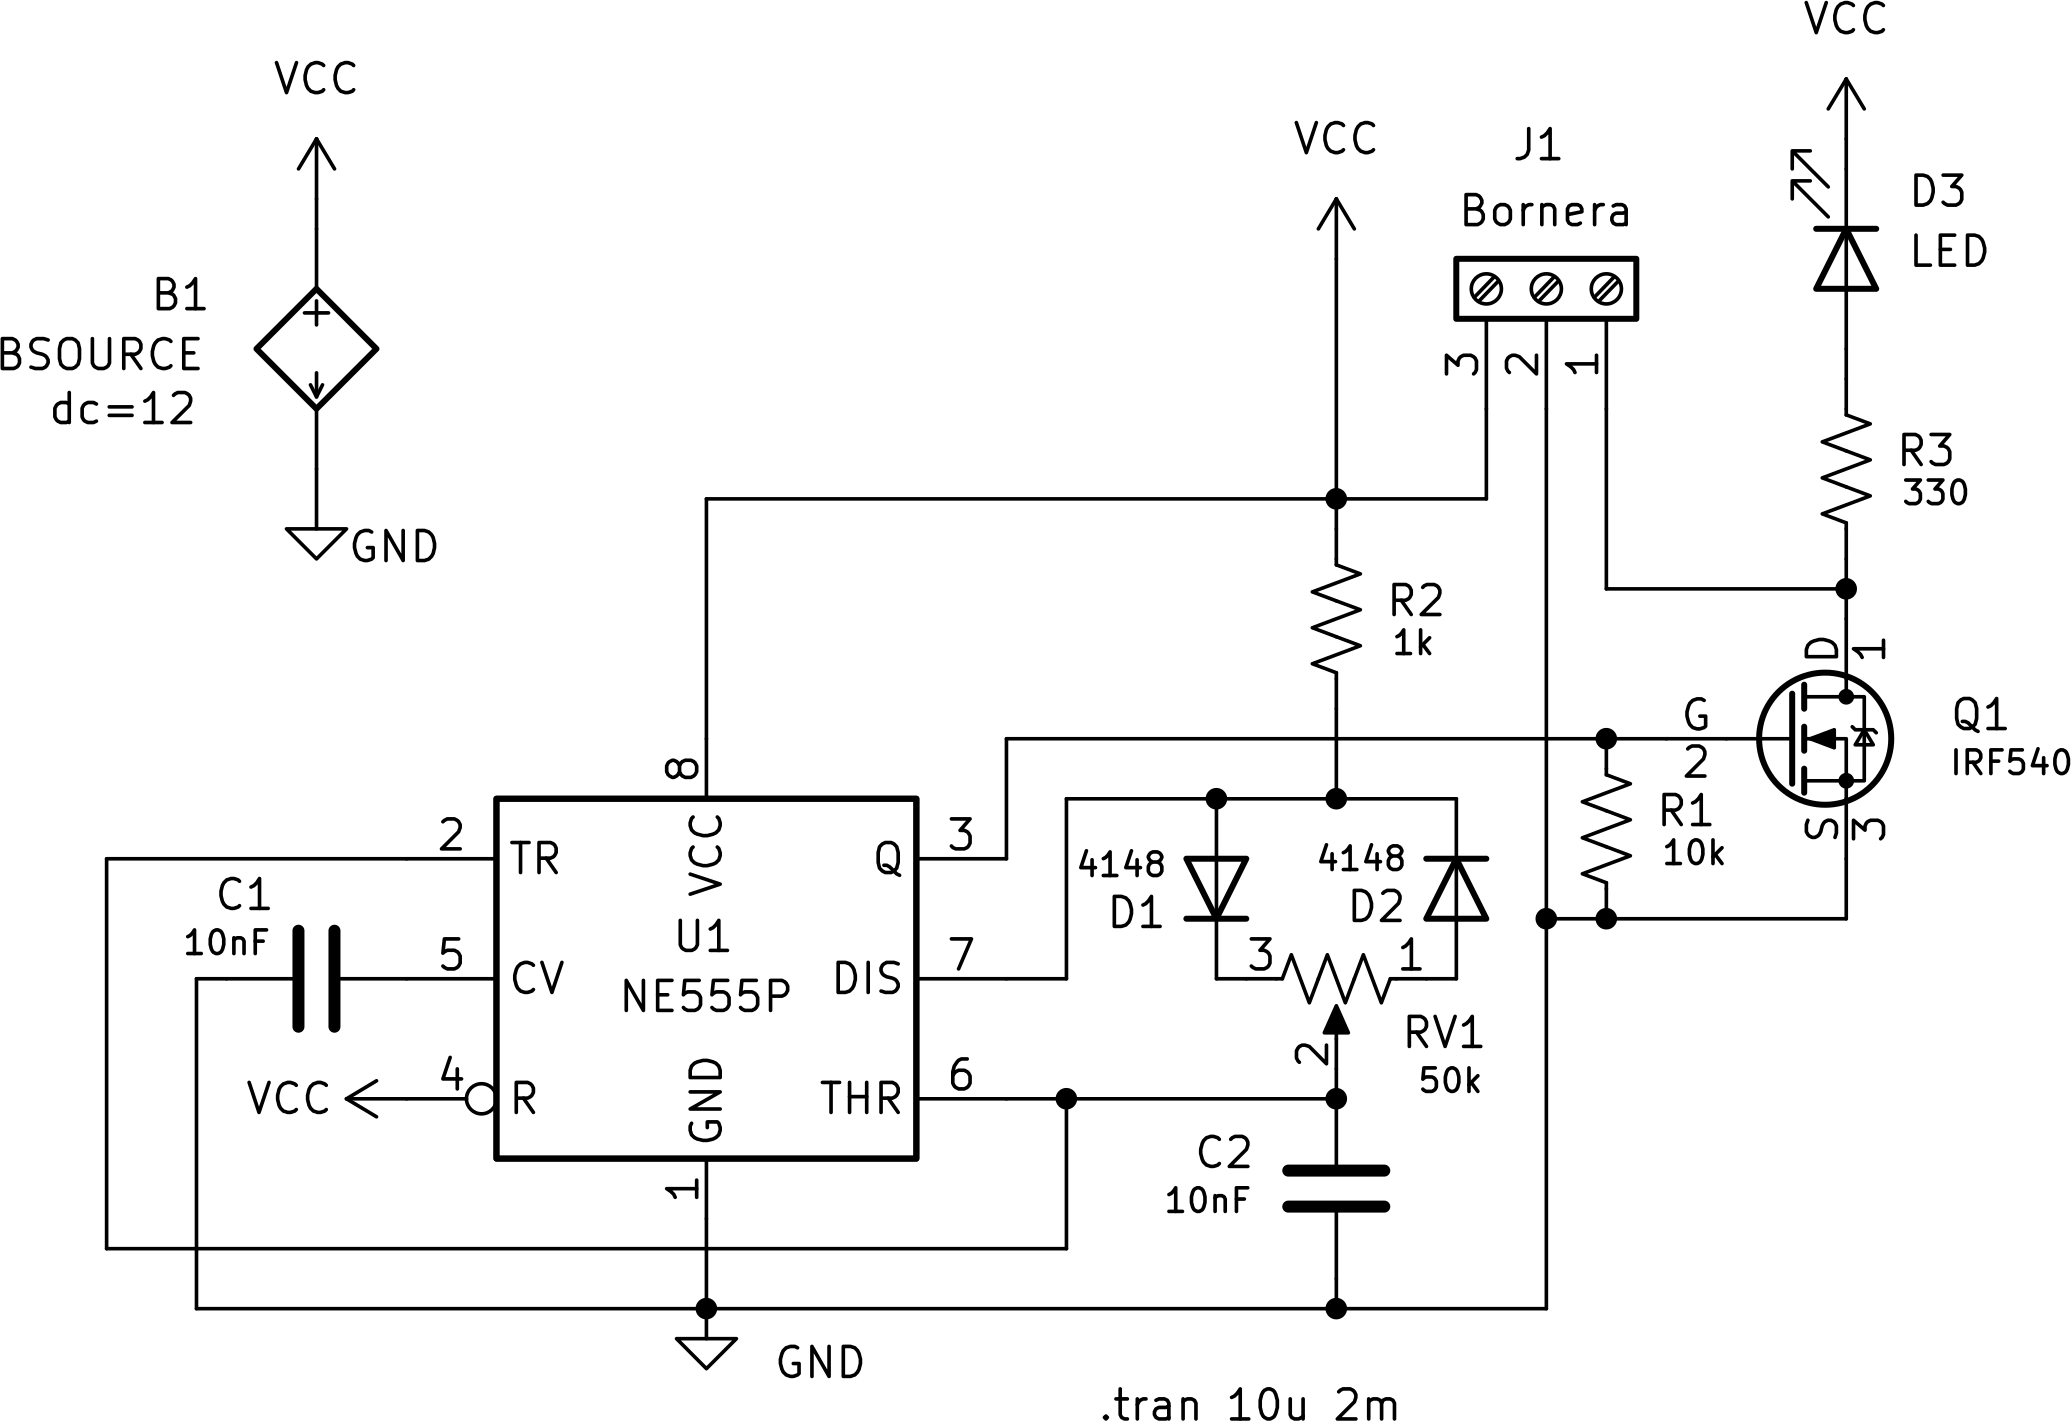
\includegraphics[width=0.75\textwidth,height=\textheight]{./esquematico.png}
\caption{Circuito Diseñado en KiCAD}
\end{figure}

\begin{figure}
\centering
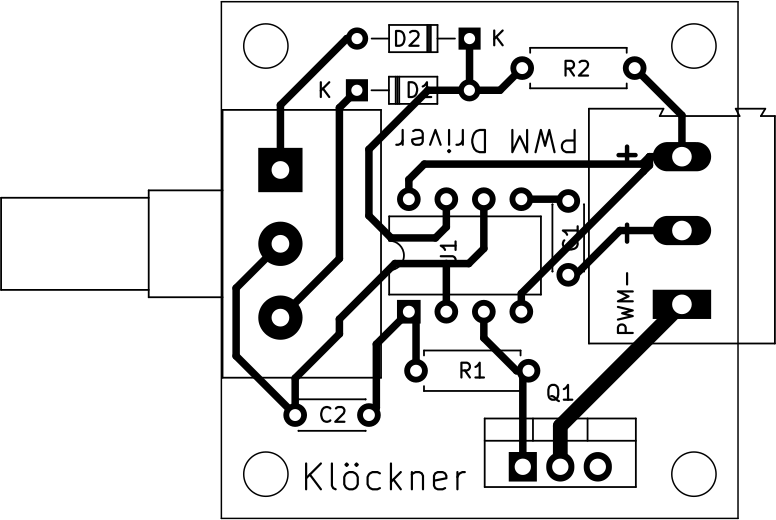
\includegraphics[width=0.6\textwidth,height=\textheight]{./pcb.png}
\caption{Diseño Placa Base a Partir del Circuito en KiCAD}
\end{figure}

\hypertarget{diseuxf1o-gabinete}{%
\subsection{Diseño Gabinete}\label{diseuxf1o-gabinete}}

\begin{figure}[!htb]%
    \centering
    \subfloat[\centering Frontal superior izquierda]{{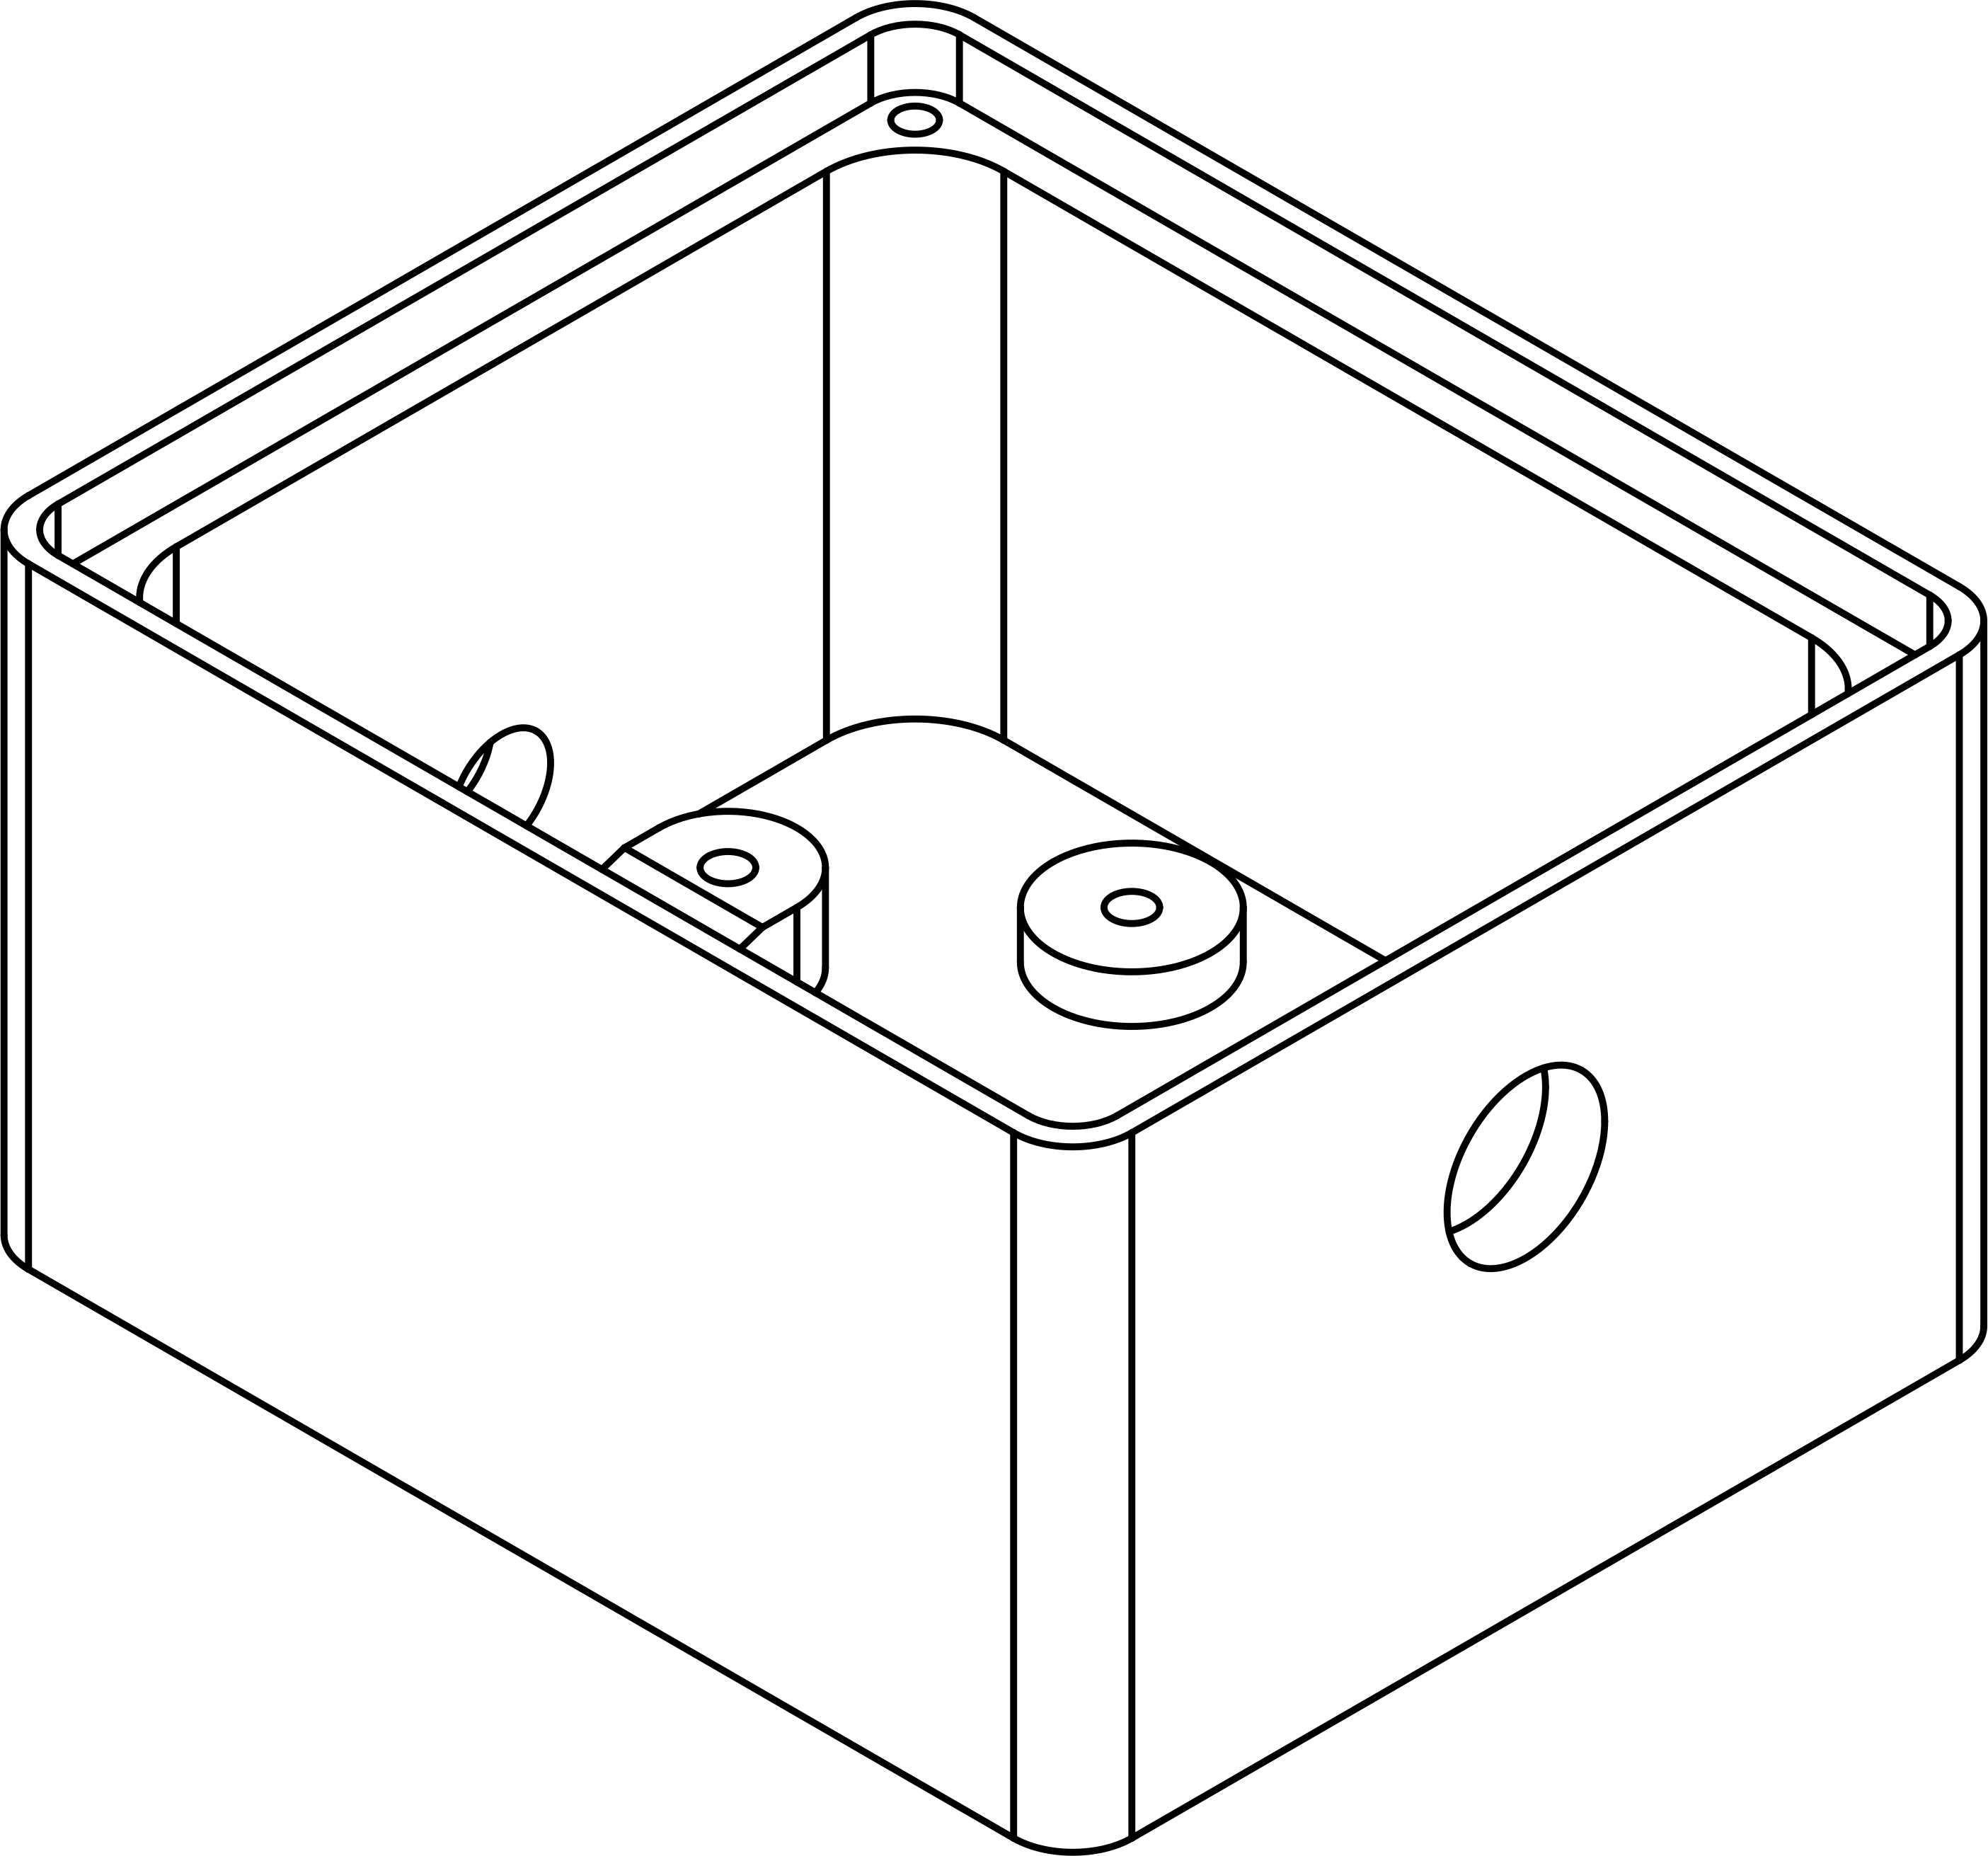
\includegraphics[width=\textwidth]{gabinete-vistas/frente-arriba-izquierda.png} }}
    \subfloat[\centering Superior]{{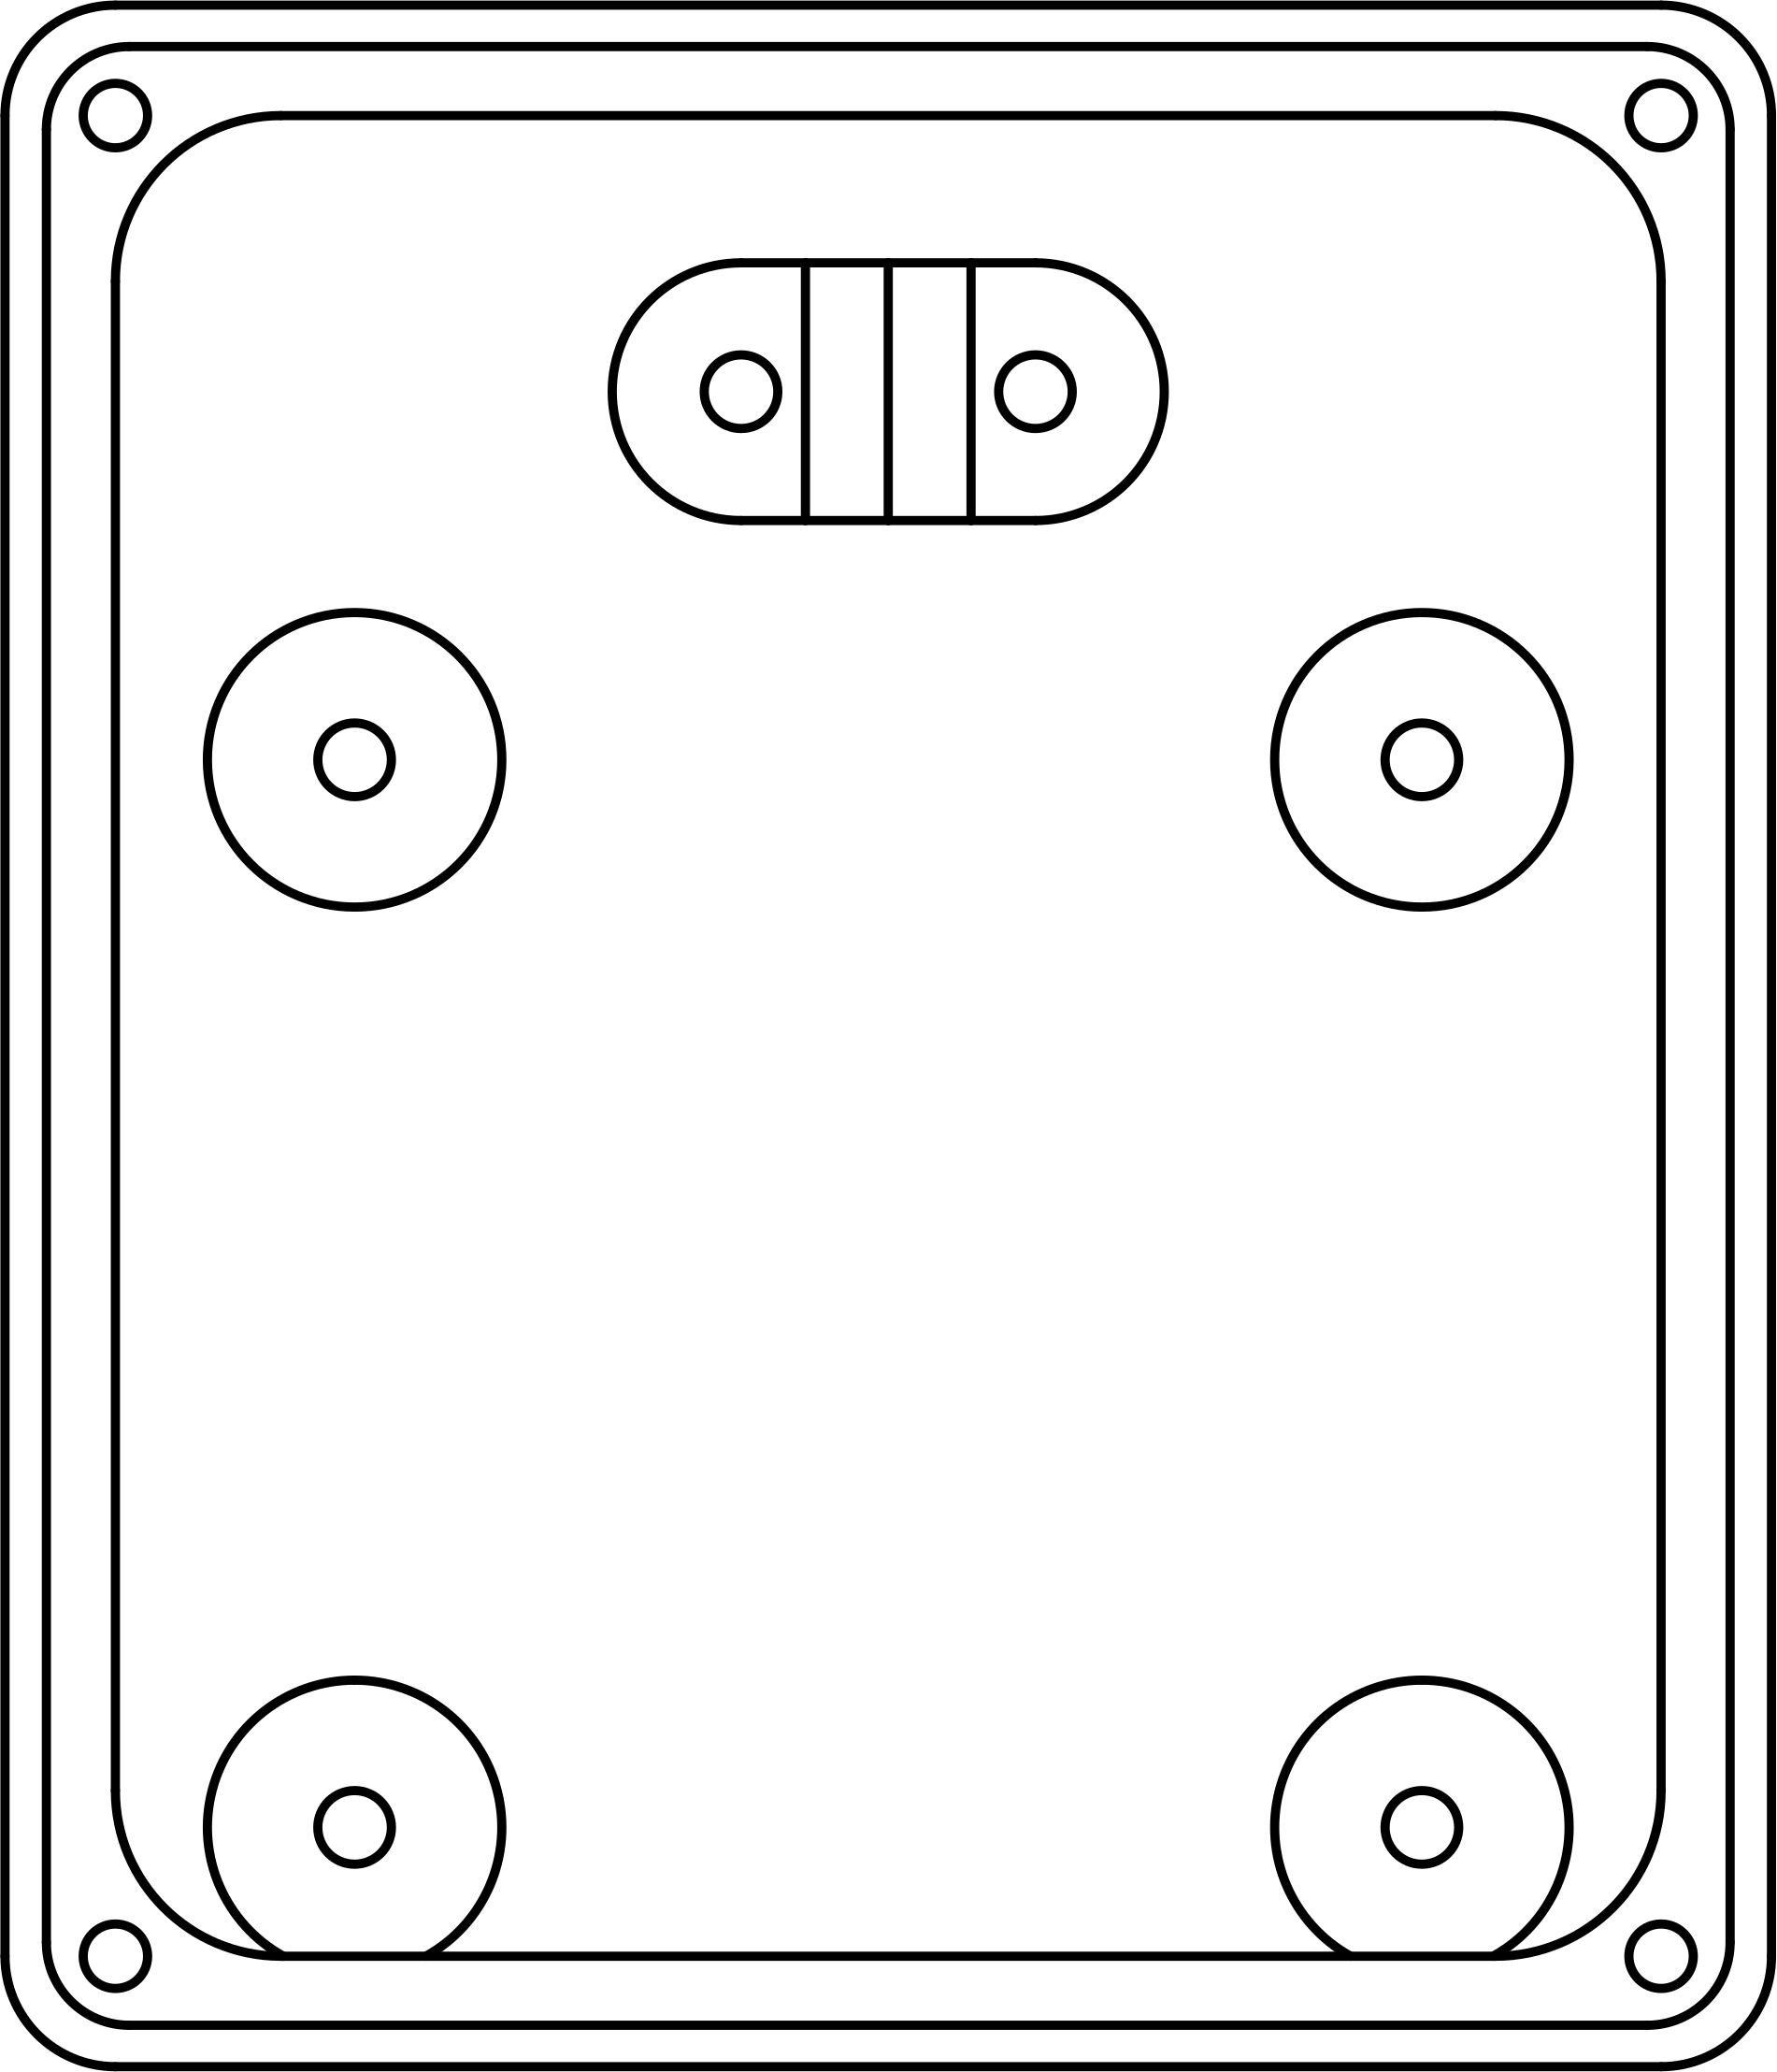
\includegraphics[width=\textwidth]{gabinete-vistas/arriba.png} }}
    \subfloat[\centering Frontal superior derecha]{{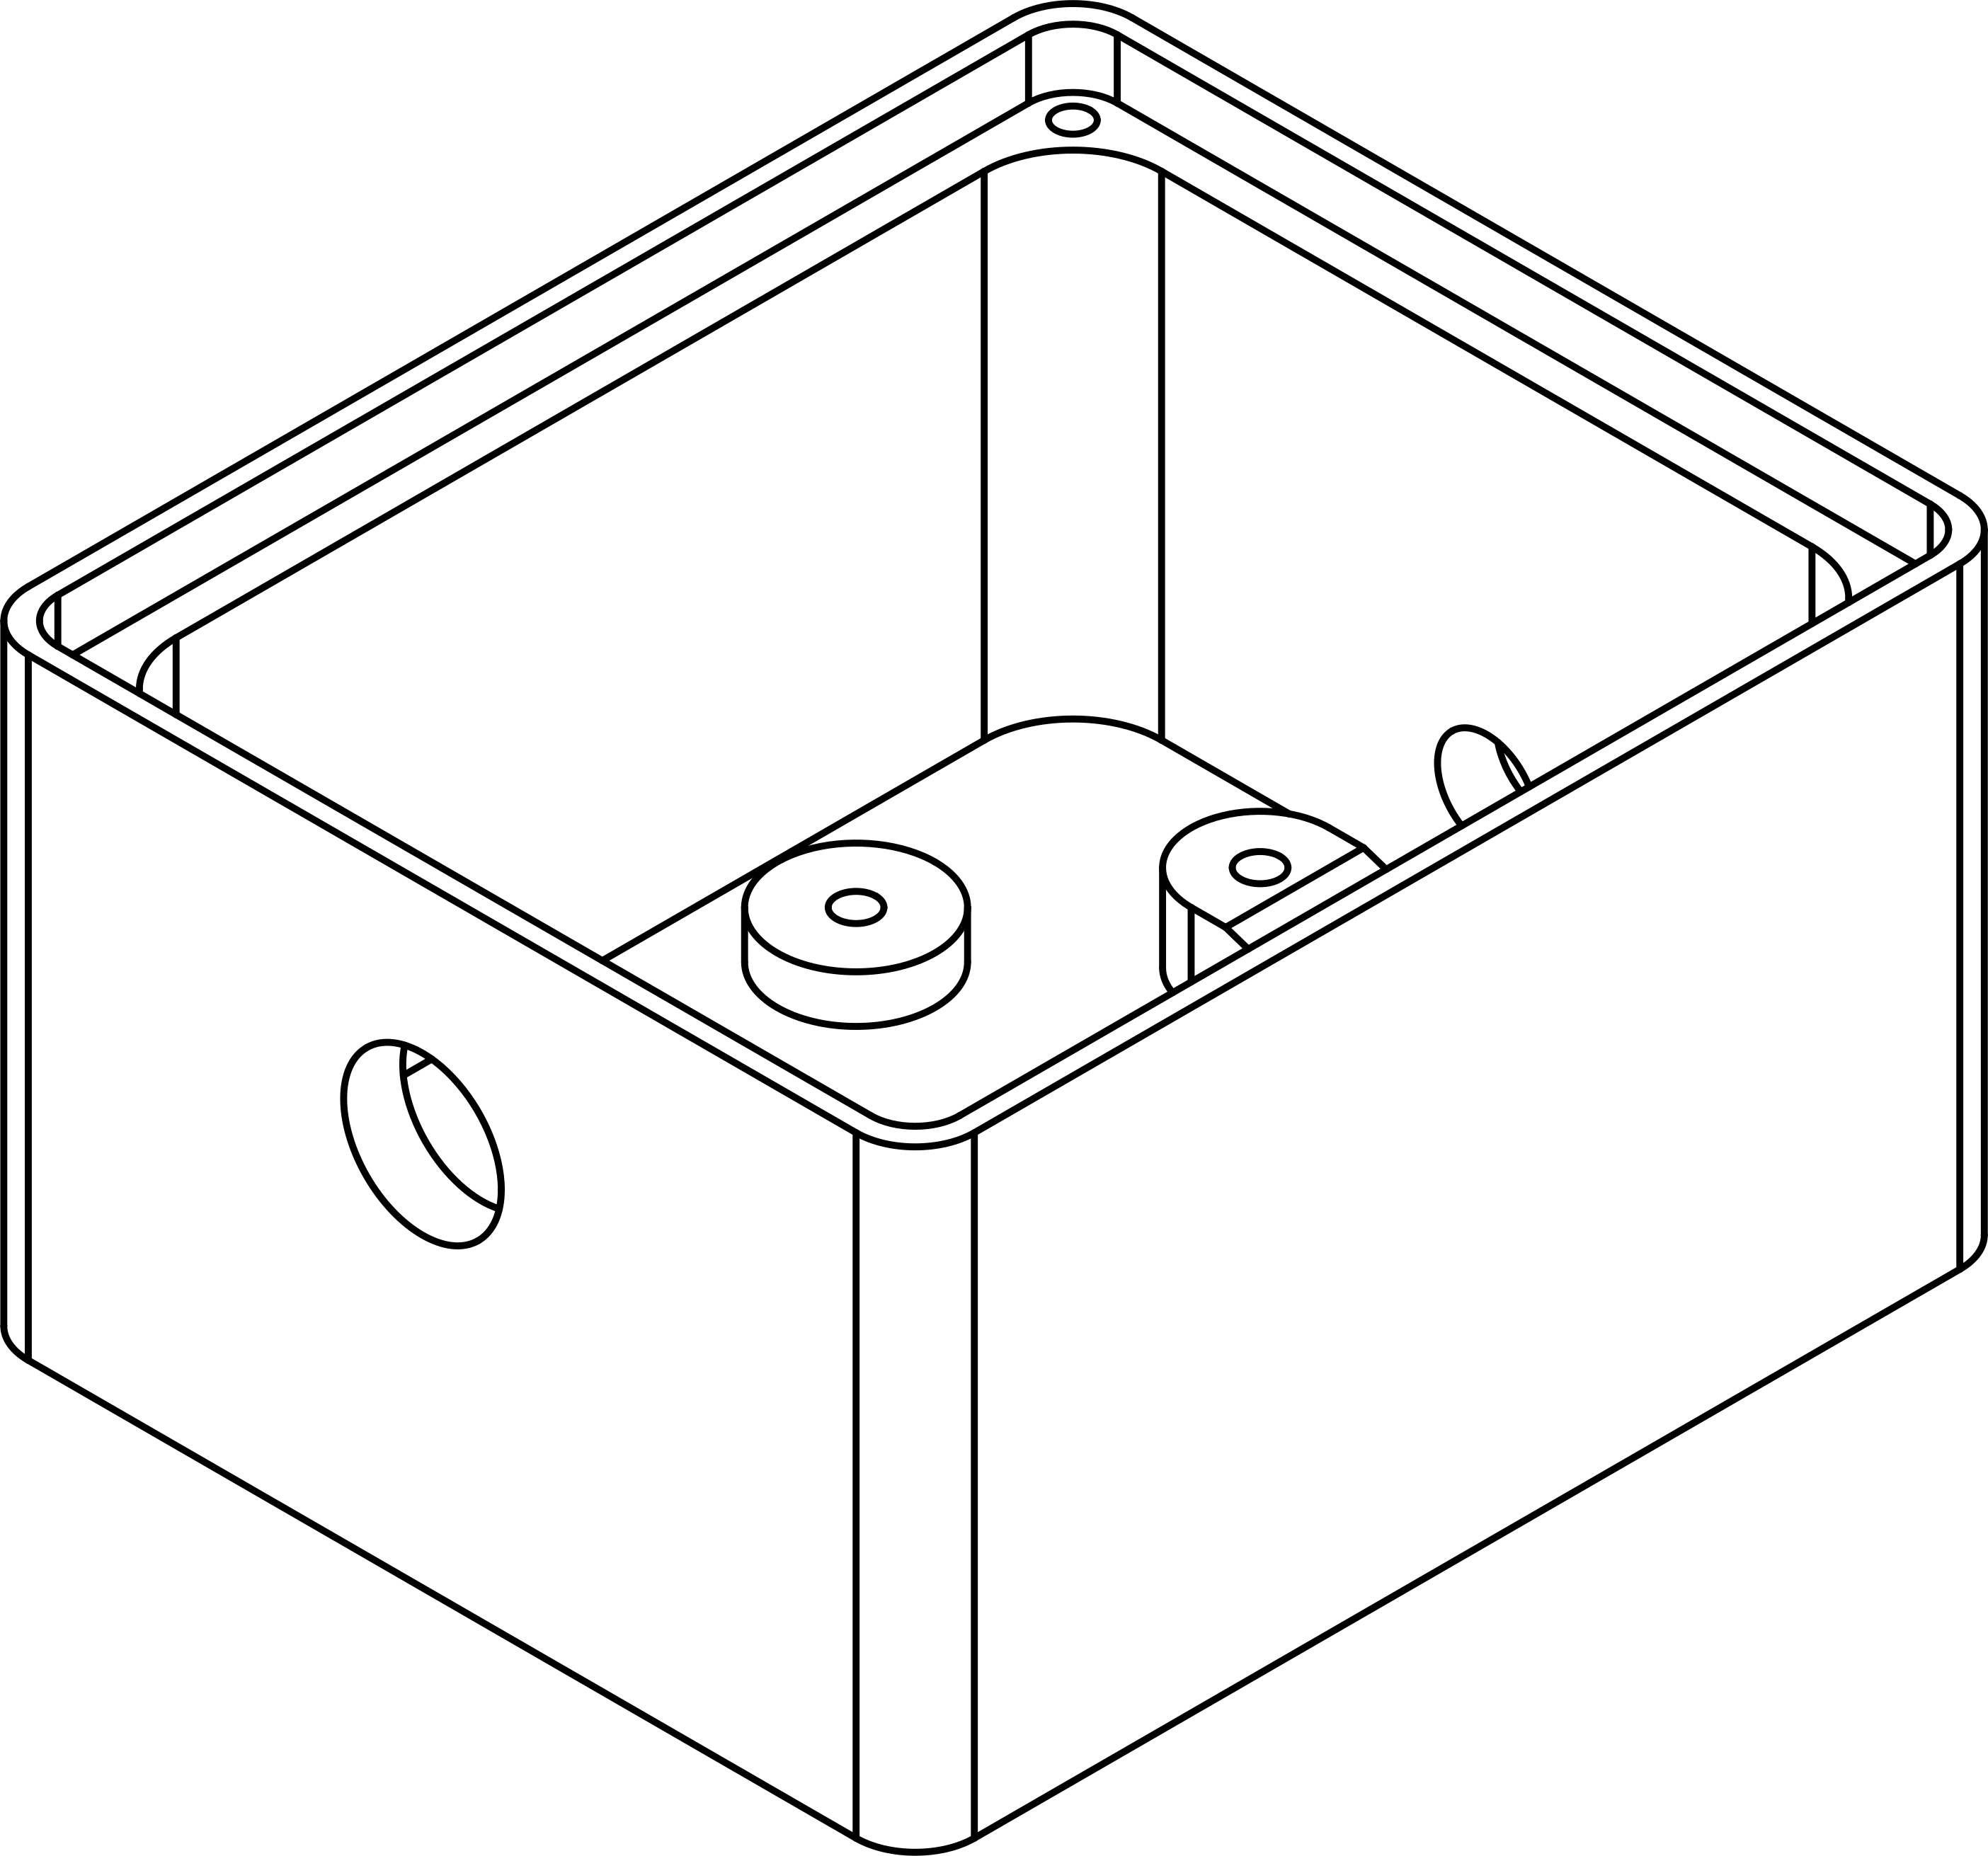
\includegraphics[width=\textwidth]{gabinete-vistas/frente-arriba-derecha.png} }}

    \centering
    \subfloat[\centering Derecha]{{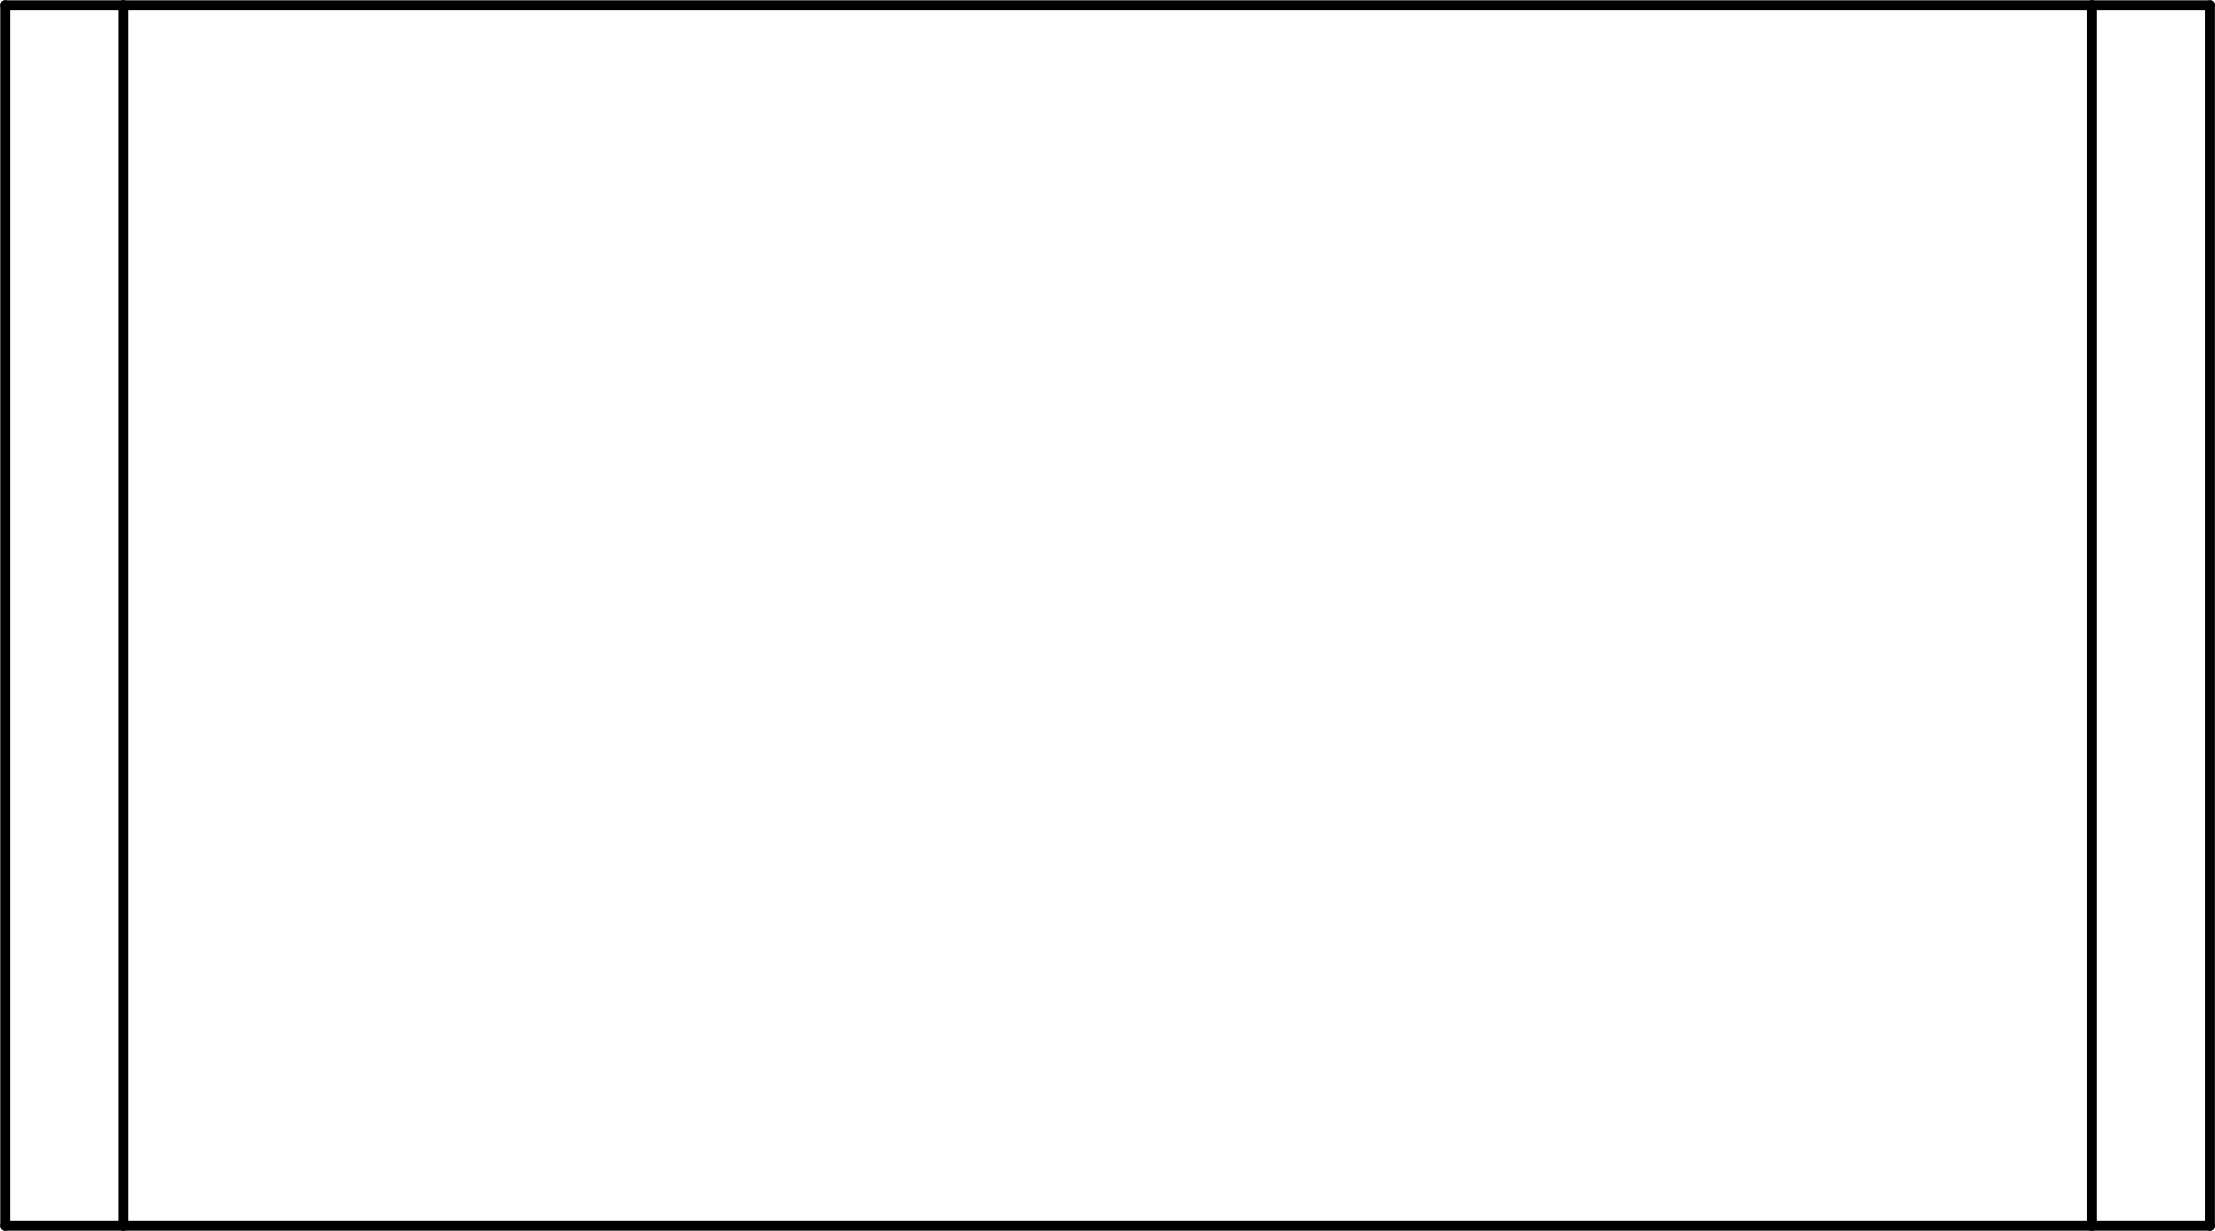
\includegraphics[width=\textwidth]{gabinete-vistas/derecha-izquierda.png} }}
    \subfloat[\centering Frontal]{{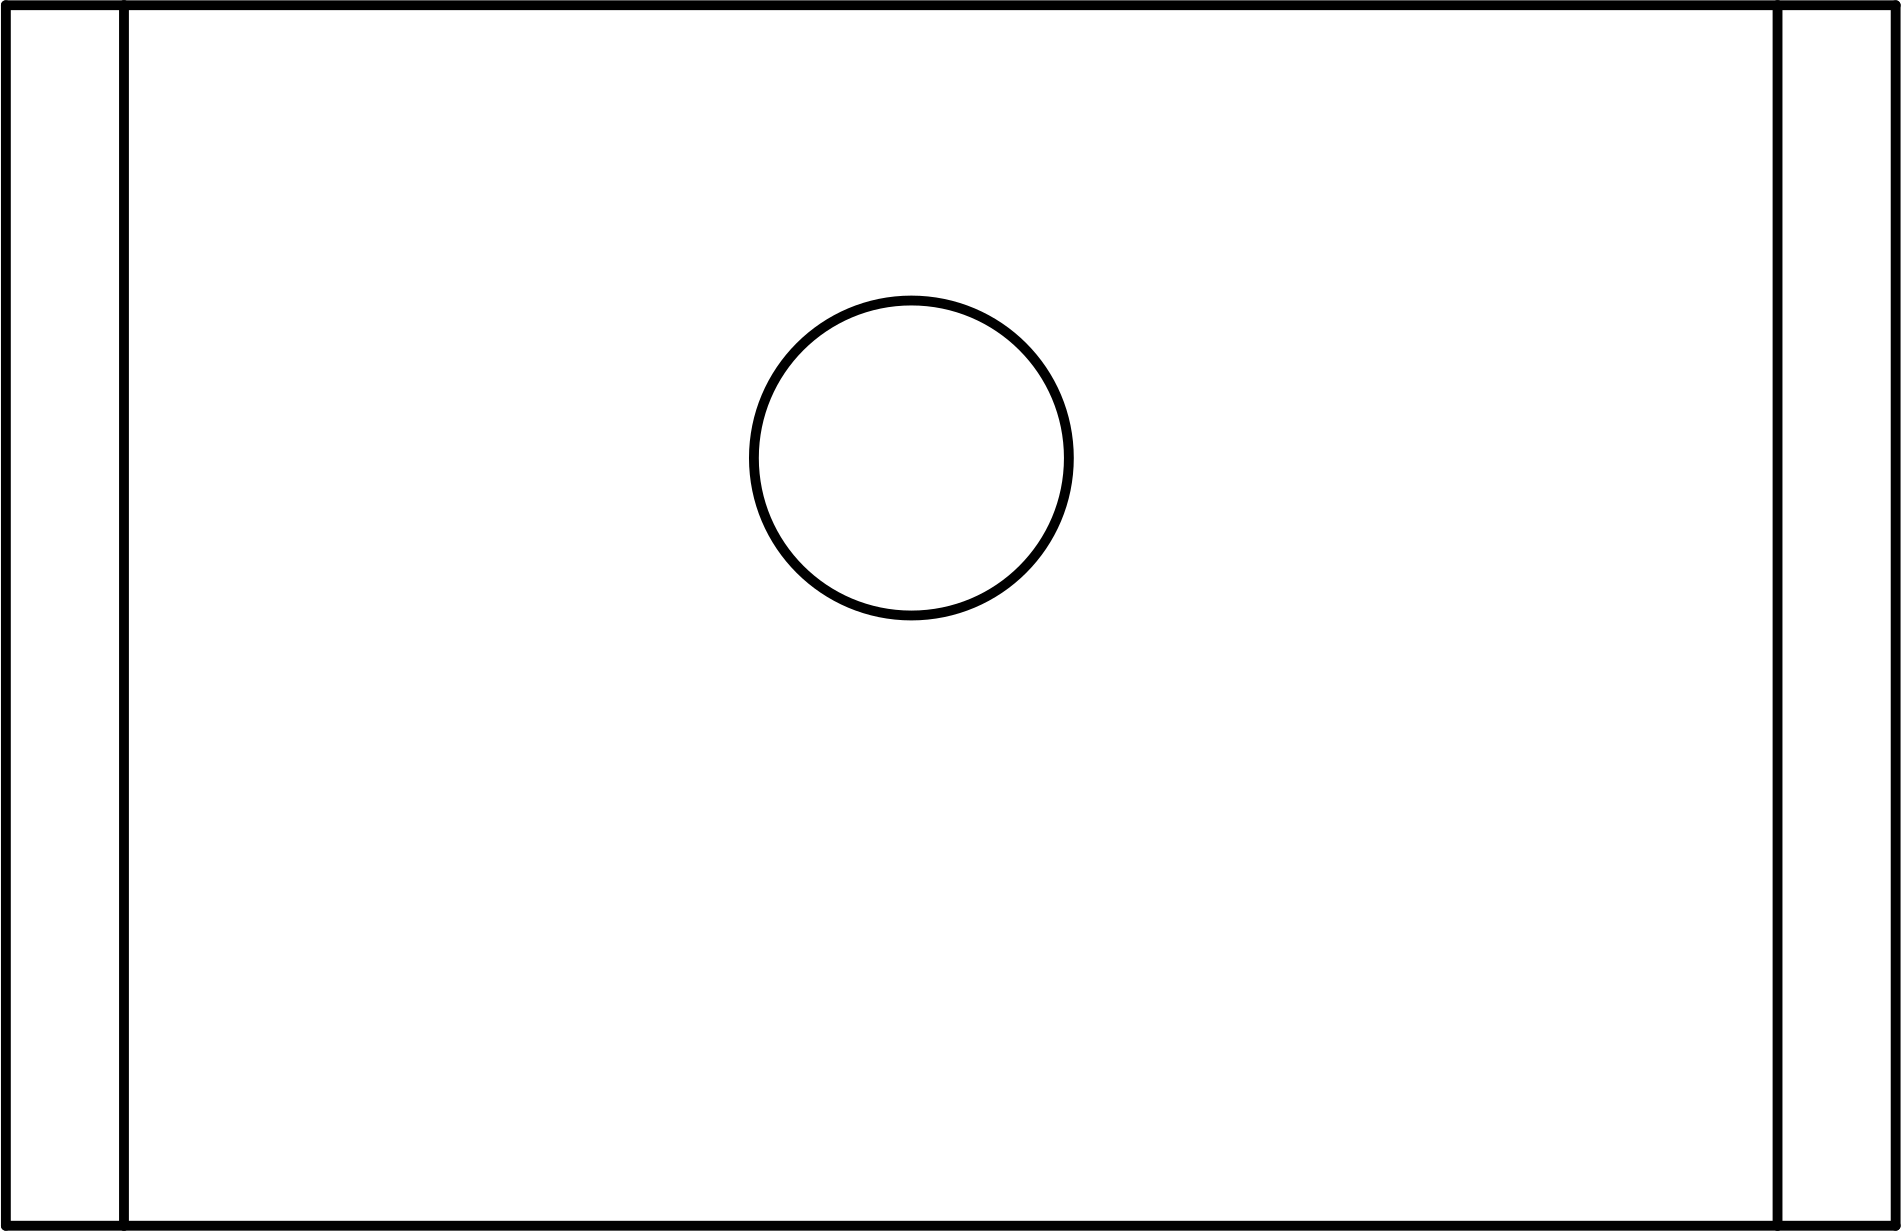
\includegraphics[width=\textwidth]{gabinete-vistas/frente.png} }}
    \subfloat[\centering Izquierda]{{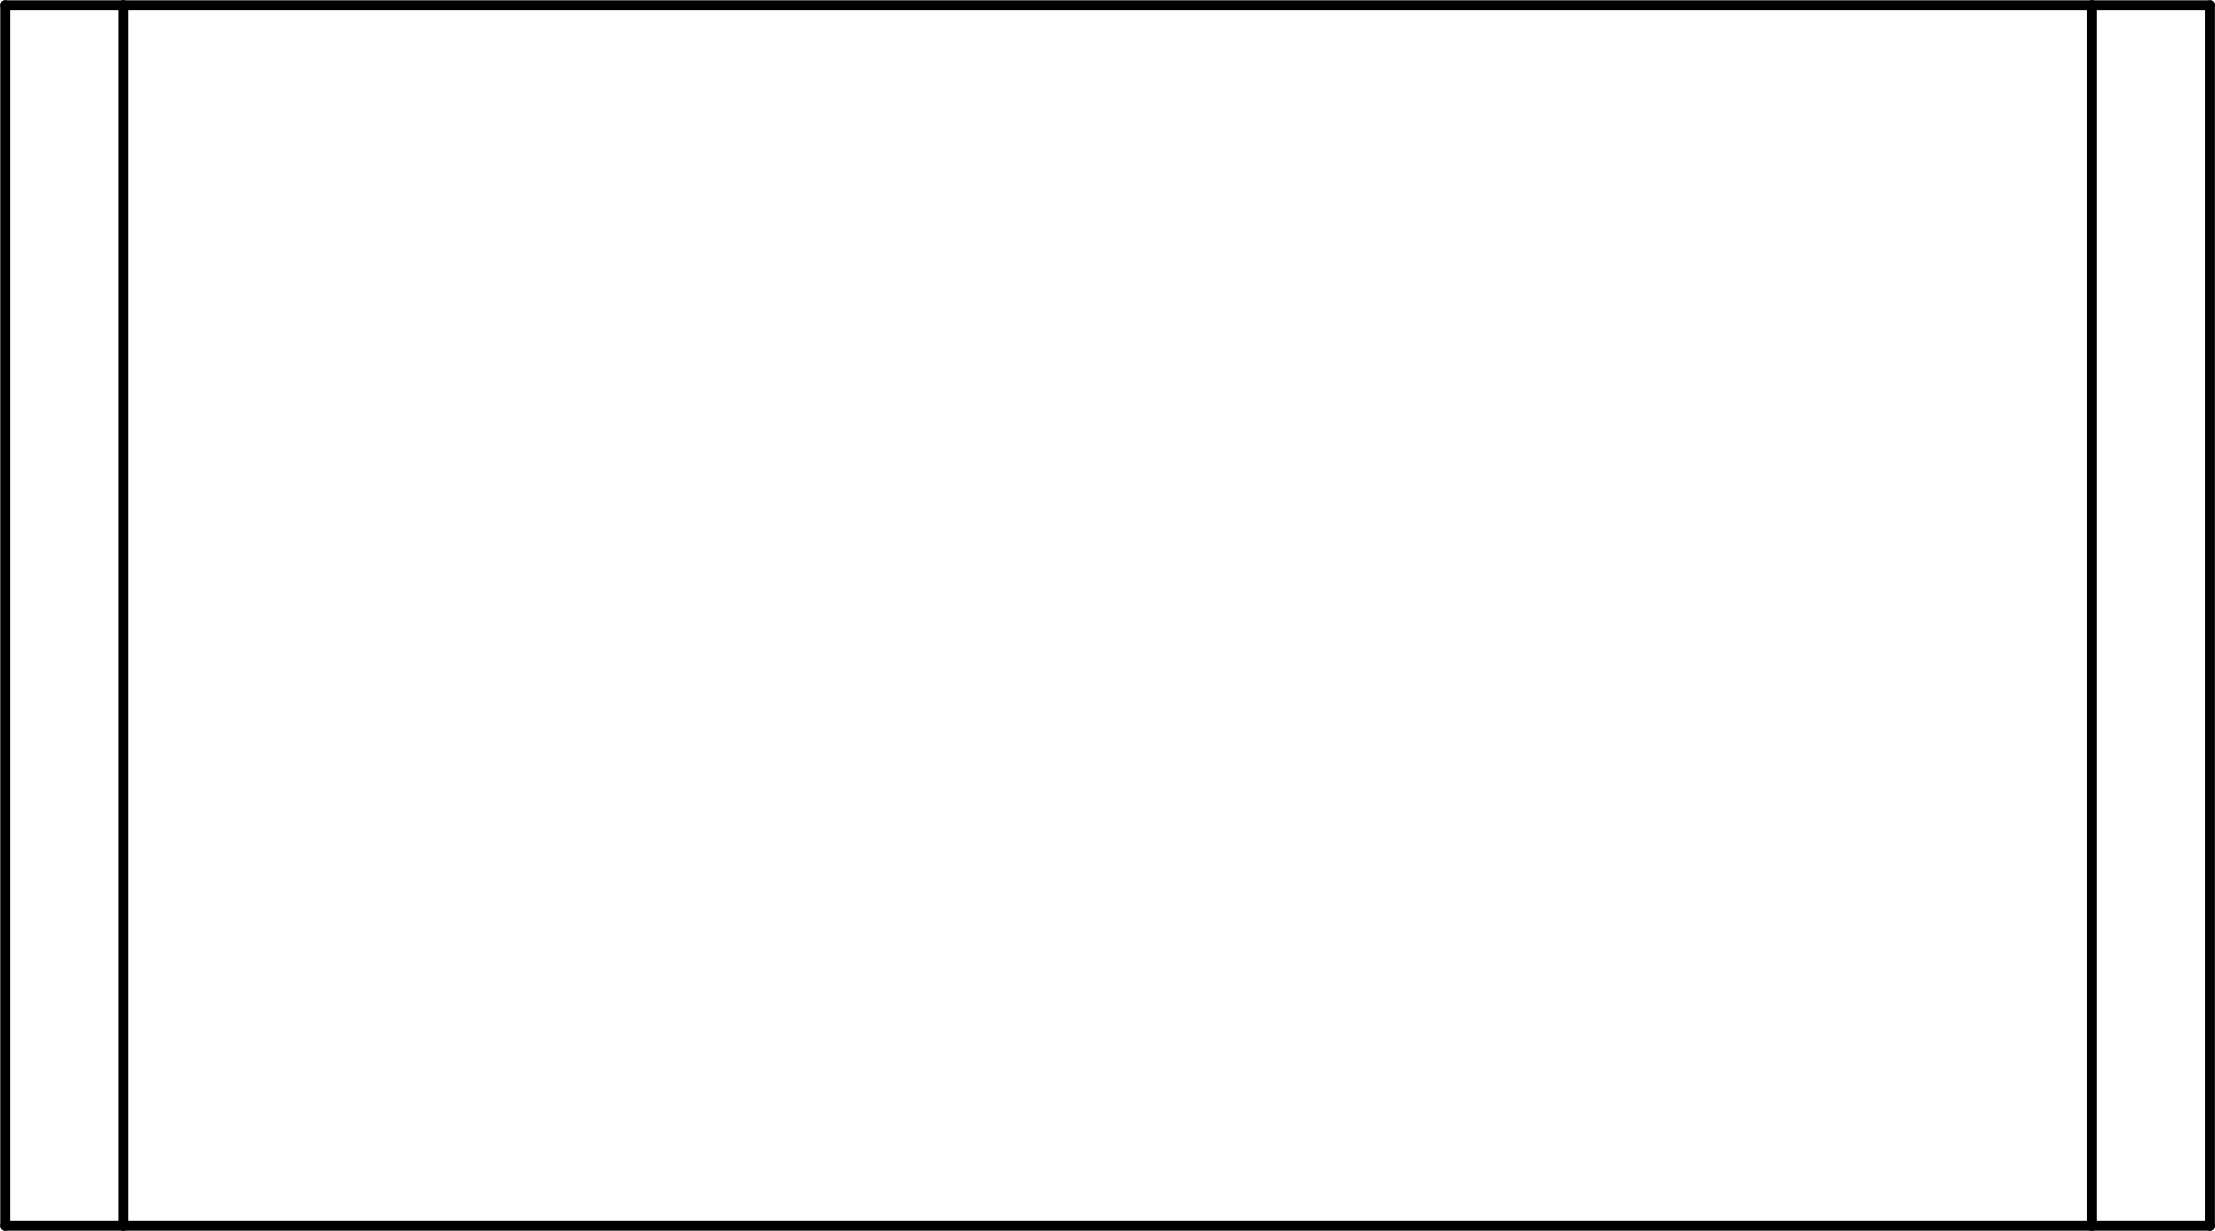
\includegraphics[width=\textwidth]{gabinete-vistas/derecha-izquierda.png} }}

    \centering
    \subfloat[\centering Frontal inferior izquierda]{{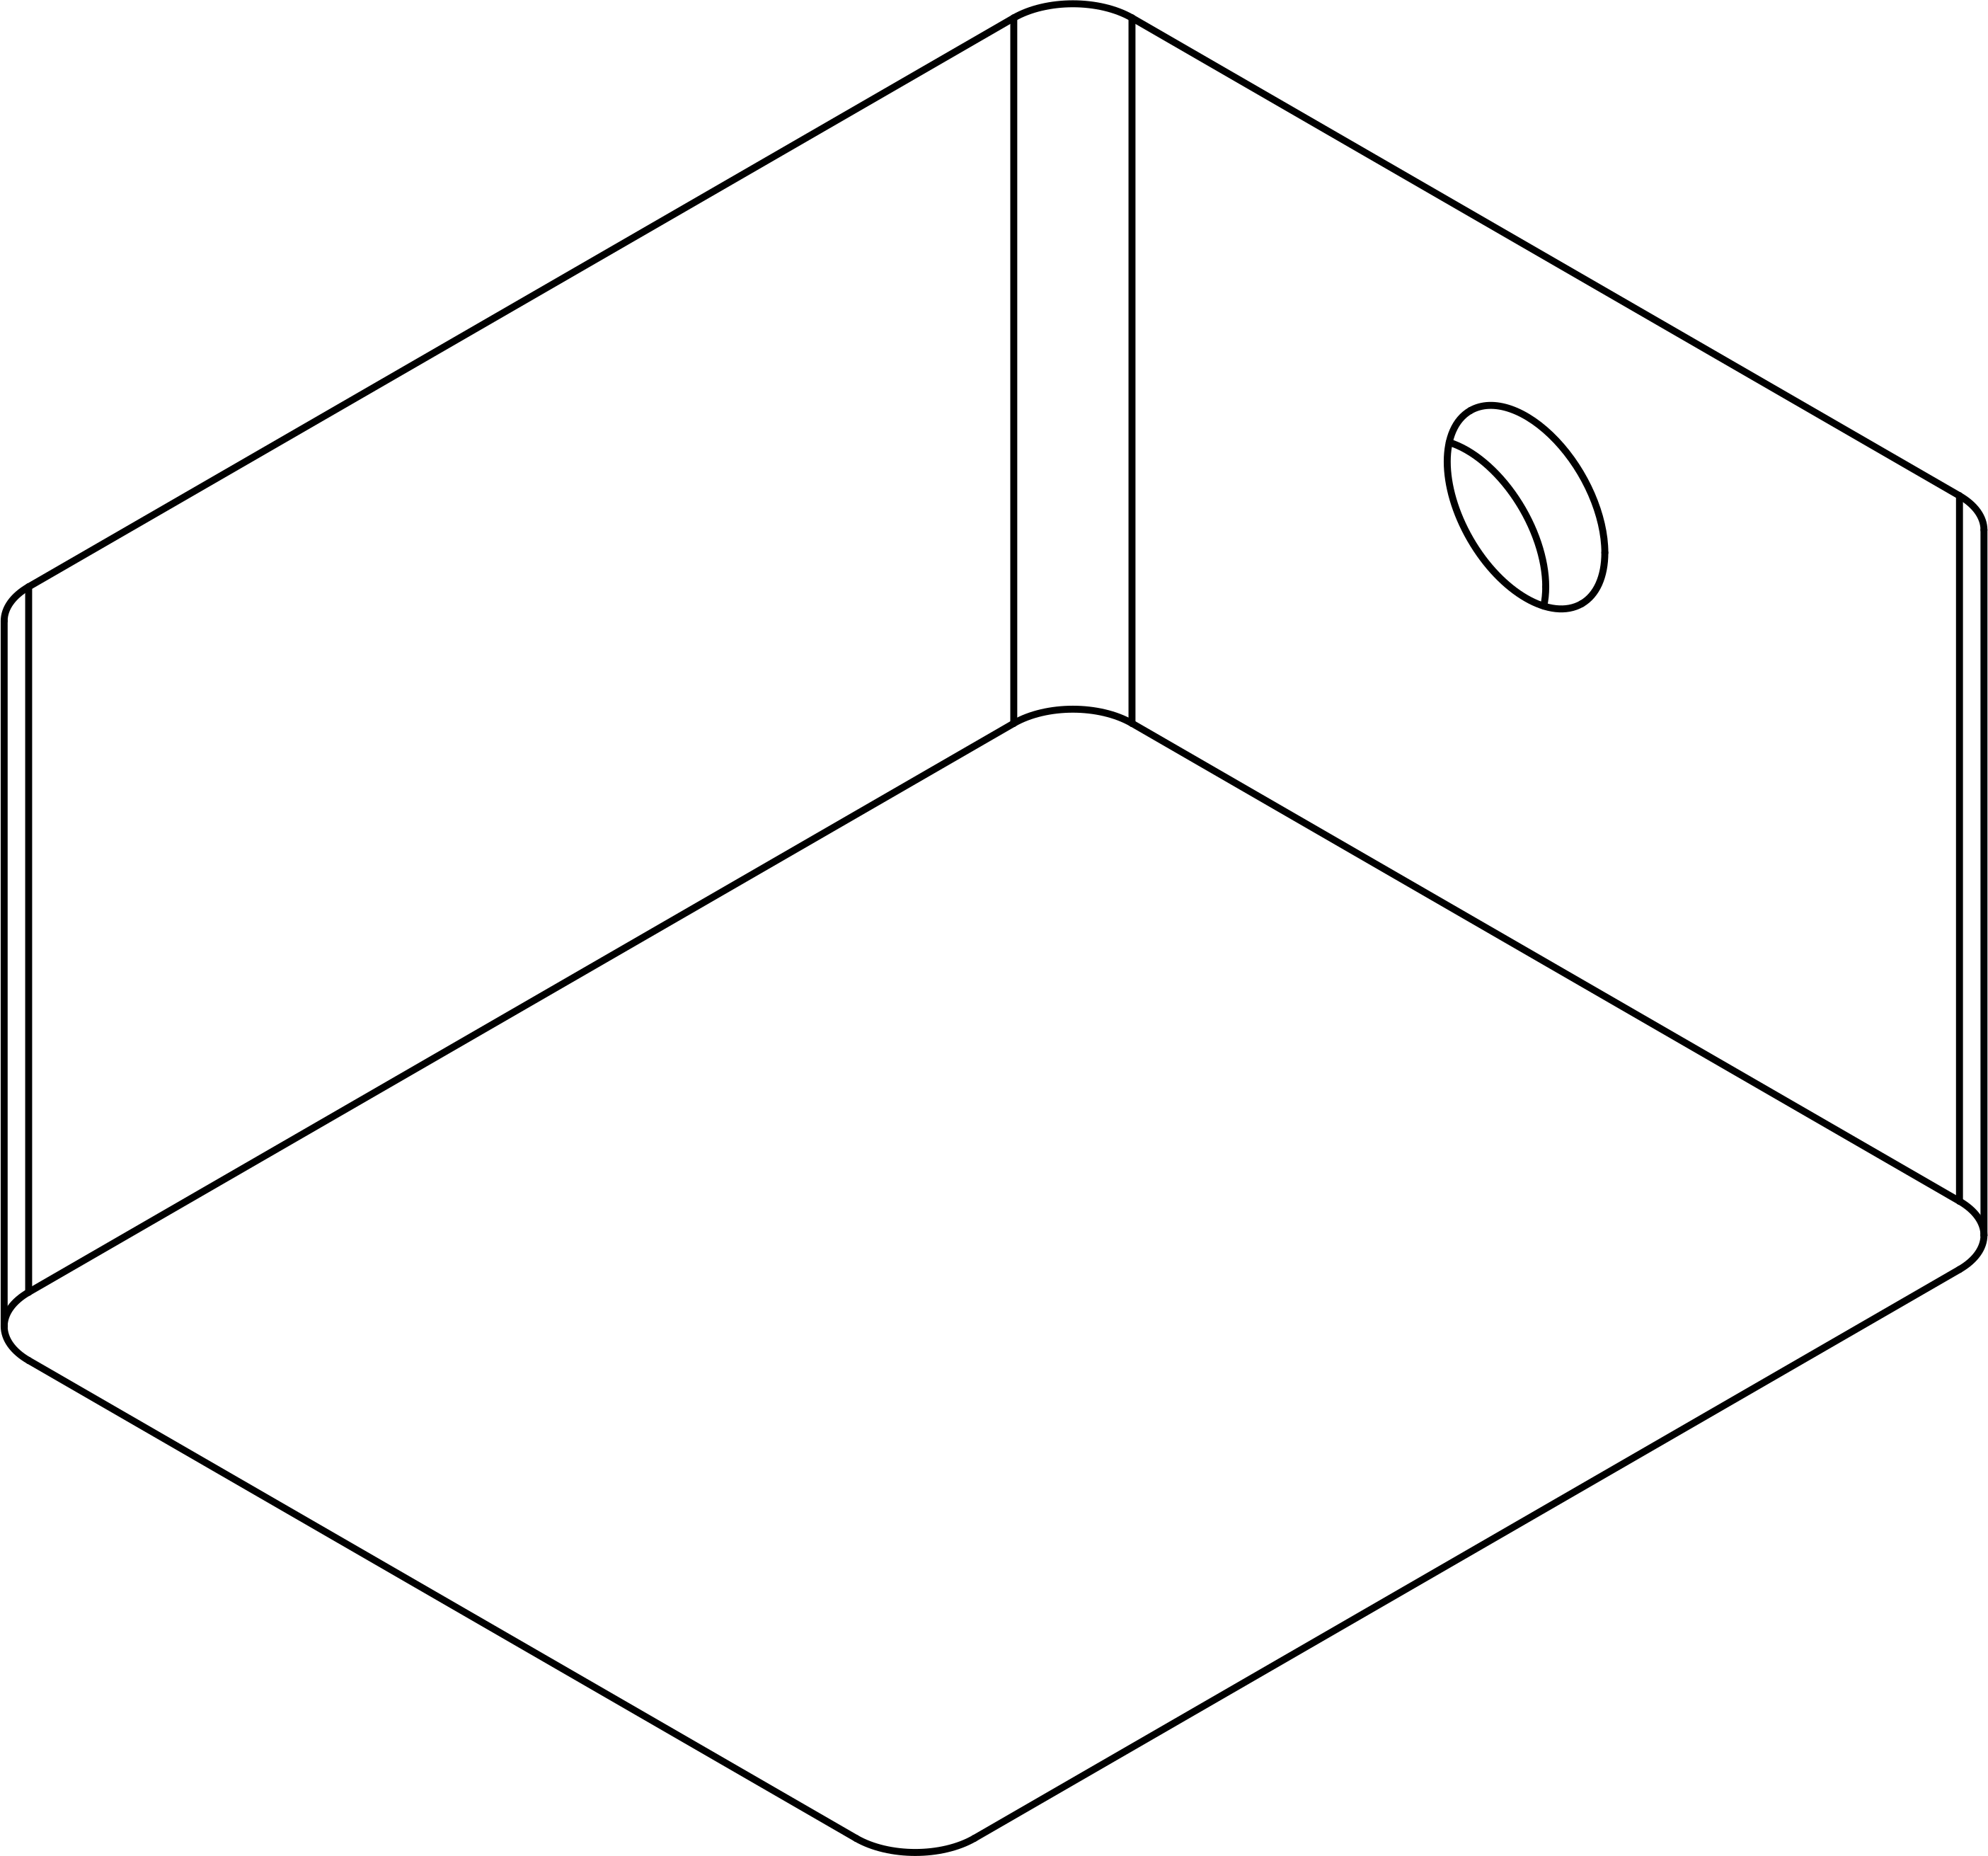
\includegraphics[width=\textwidth]{gabinete-vistas/frente-abajo-izquierda.png} }}
    \subfloat[\centering Inferior]{{
\includegraphics[width=\textwidth]{gabinete-vistas/abajo.png} }}
    \subfloat[\centering Frontal inferior derecha]{{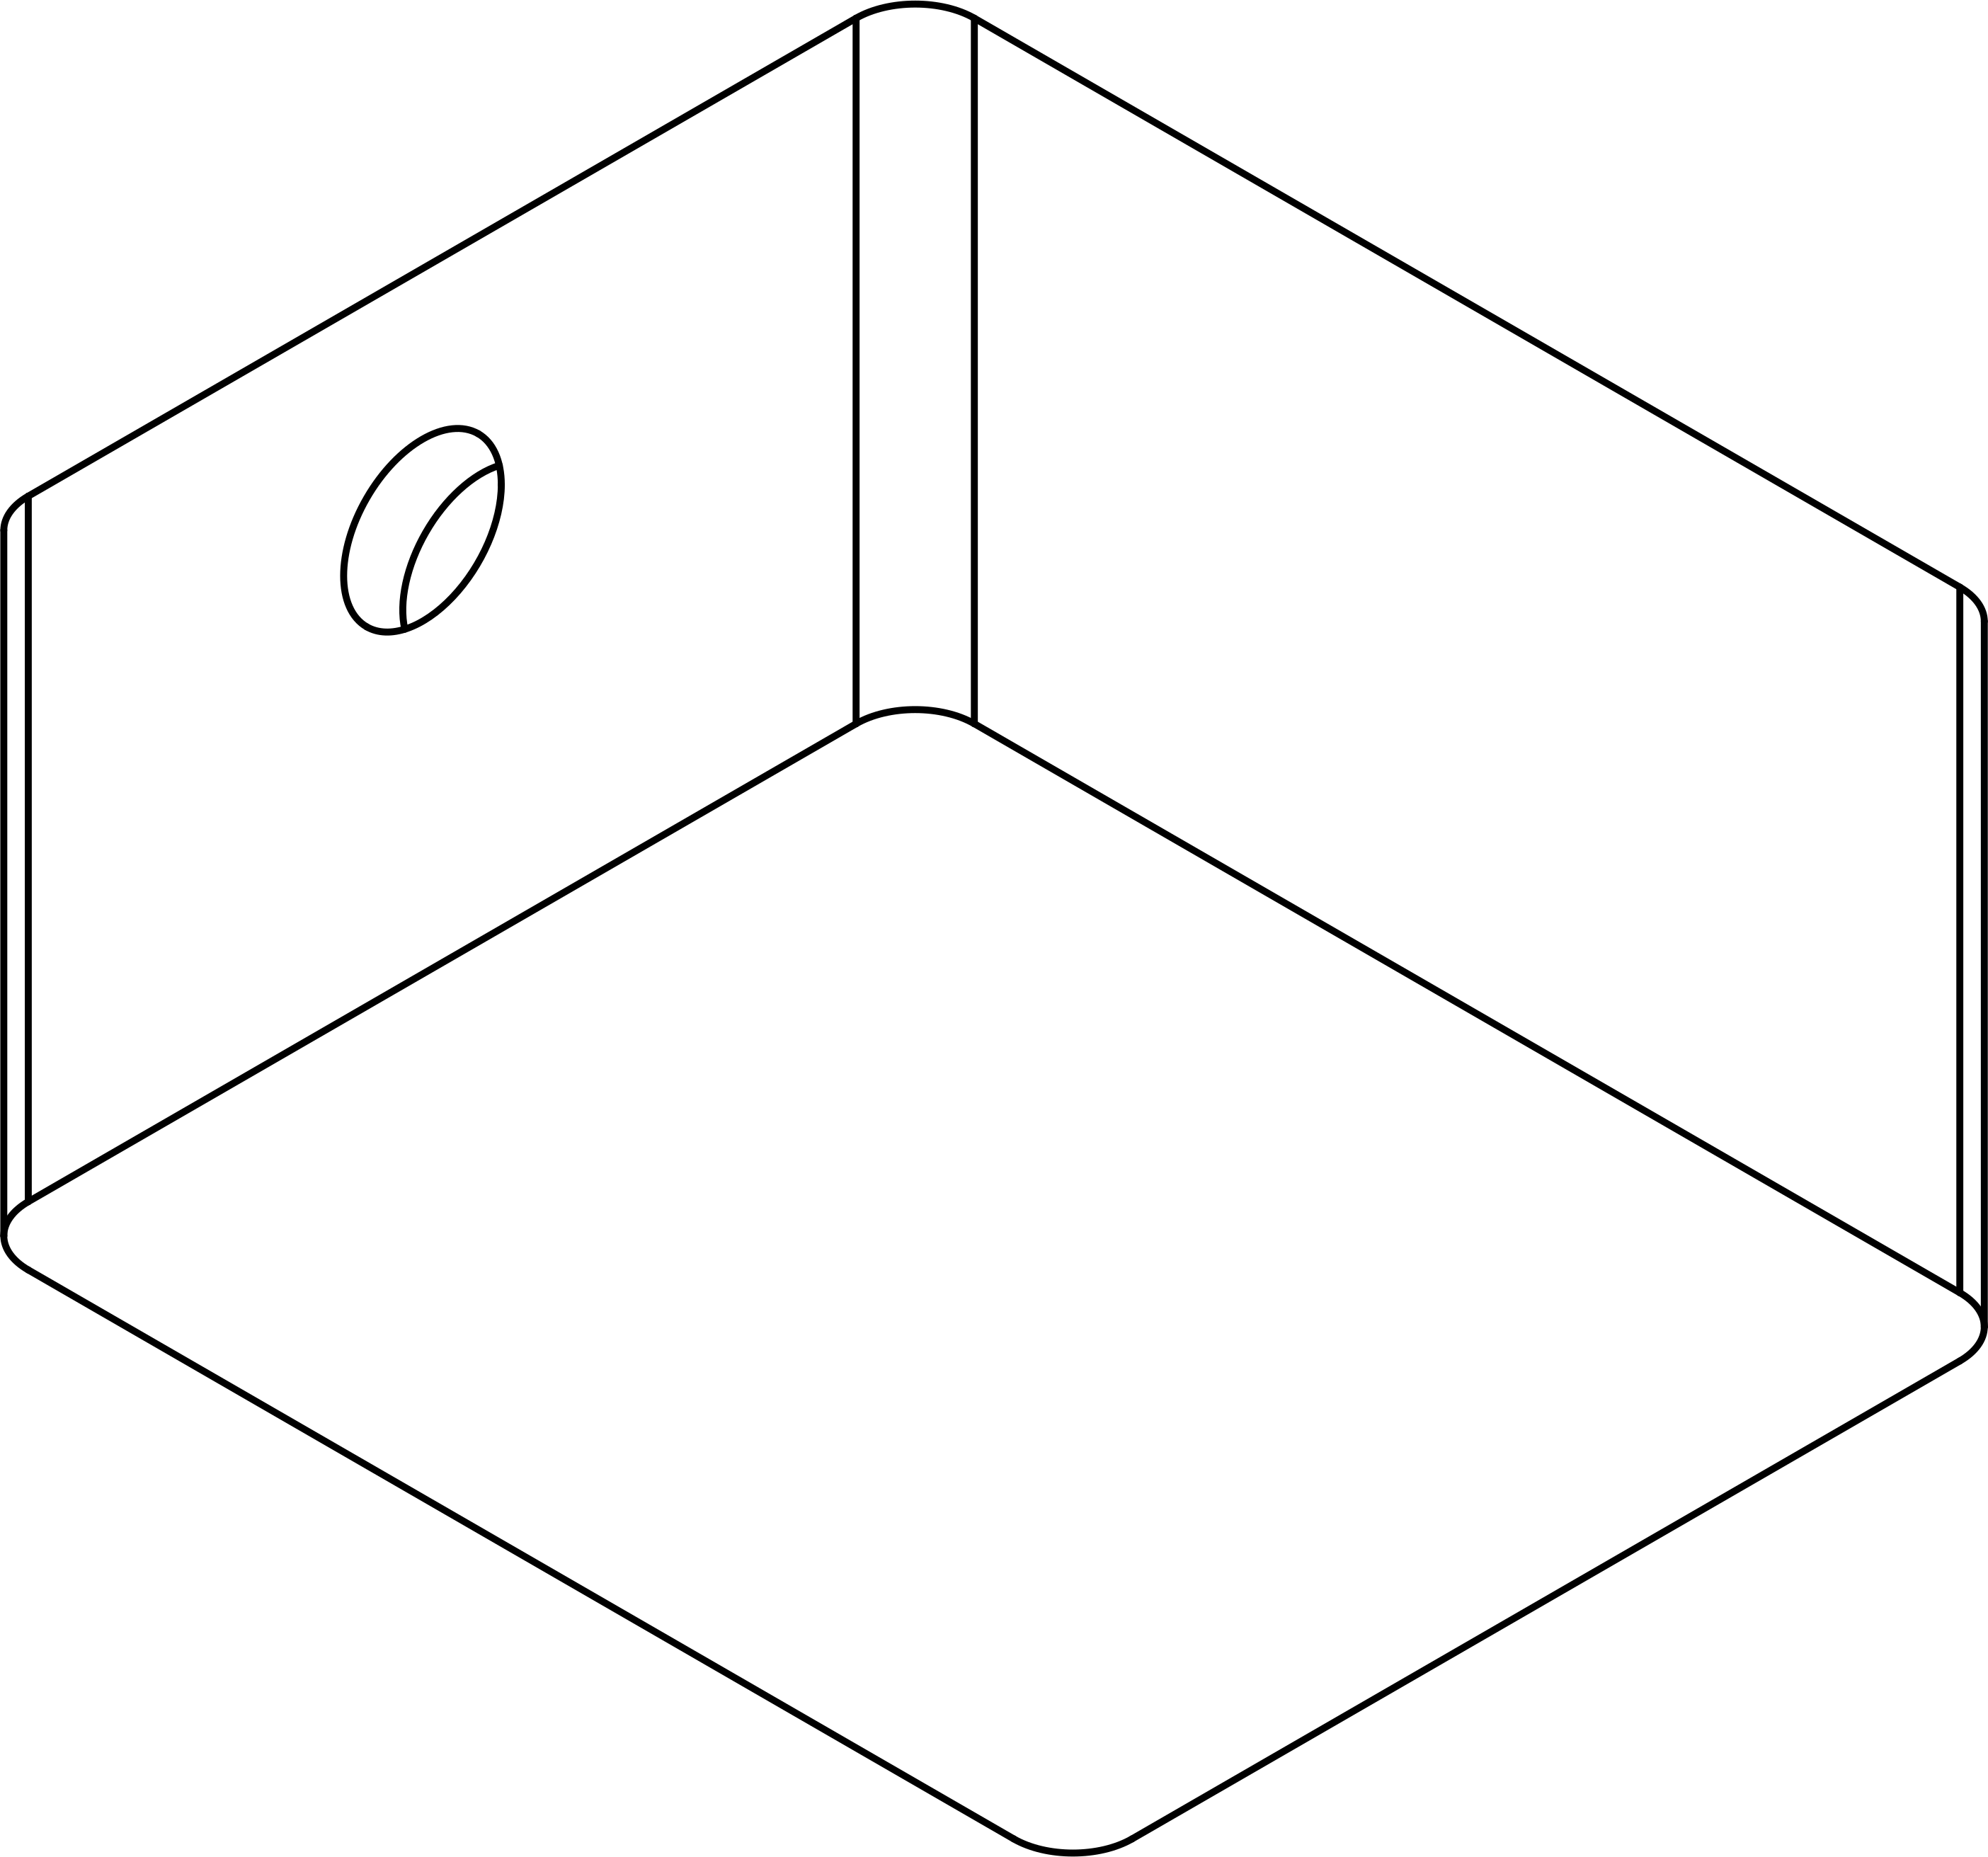
\includegraphics[width=\textwidth]{gabinete-vistas/frente-abajo-derecha.png} }}
    \caption{Vistas del Gabinete Modelado Utilizando FreeCAD}
\end{figure}

\hypertarget{construccion-de-la-placa-base}{%
\subsection{Construccion de la Placa
Base}\label{construccion-de-la-placa-base}}

\hypertarget{consideraciones}{%
\subsubsection{Consideraciones}\label{consideraciones}}

Por la resistencia R2 circulan aproximadamente \(11 mA\) según
simulación independientemente de la carga, esta corriente circula cuando
el capcacitor C2 se descarga. Esta corriente provoca que la resistencia
R2 cuyo valor es \(1000\ \Omega\) deba disipar
\(V_{CC}\frac{R2}{R2+RV1}\cdot 11mA\), siendo \(RV1\) el valor del
potenciometro. Para el potenciometro en un \(50\%\), la potencia
disipada por R2 resulta:

\[P=12V\cdot \frac{1000\Omega}{1000\Omega + 25000\Omega} \cdot 11mA = 5mW\]

Por lo que con un resistor que soporte potencia de \(0.25W\) resulta mas
que suficiente.

\hypertarget{materiales}{%
\subsubsection{Materiales}\label{materiales}}

\begin{itemize}
\tightlist
\item
  1x Reistencia \(1k\Omega\)
\end{itemize}

\end{document}
